\documentclass[a4paper,12pt]{article}
 \usepackage[italian]{babel} 
\usepackage{graphicx}
\usepackage{caption}
\usepackage{geometry}
\usepackage{enumitem}
\usepackage{fancyhdr}
\usepackage{svg-extract}
\usepackage{hyperref}
\usepackage[nottoc]{tocbibind}



\geometry{a4paper, top=1.5cm, bottom=1.5cm, left=1.5cm, right=1.5cm, }
\setlength{\parindent}{0pt} %\setlength{\parskip}{0,25cm plus1mm minus1mm}
\graphicspath{ {images} } 
\lhead{
\includegraphics[width=5cm]{logounitn.jpg}}
\rhead{
\includegraphics[width=3cm]{logolifemanager.png}}
\setlist[itemize]{leftmargin=5.5mm}







%\fancyhead[L]{
\includegraphics[width=5cm]{logounitn.jpg}}
\renewcommand{\headrulewidth}{0pt}
\raggedbottom

%-----------------------------------------TITOLO
 \title{LifeManager}
 \author{
 Corso di Ingegneria del software\\ \\Luca Boschiero, Mauro Meneghello, Nicola Turniano
 }
 \begin{document} 
 \maketitle
 \thispagestyle{fancy}
 %-----------------------------------------INFORMAZIONI STUD
 \vspace{15cm}
\hrule
\begin{table}[!h] 
\begin{tabular}{l l l}
Gruppo T10\\
Deliverable 2\\
 \\
Mauro Meneghello & 217564 & mauro.meneghello@studenti.unitn.it \\
Luca Boschiero & 217460 & luca.boschiero@studenti.unitn.it \\
Nicola Turniano  & 271457 & nicola.turniano@studenti.unitn.it \\
\end{tabular}
\end{table}
\hrule



  

\newpage
 %-----------------------------------------SVOLGIMENTO


\part{Analisi dei componenti}
Nel seguente capitolo analizzeremo i componenti interni che costituiranno il nostro sistema, andando a definire una prima architettura al software {\scshape LifeManager}, e le relazioni tra questi componenti. 

In particolare, un componente rappresenta un’entità autonoma all’interno di un sistema o sottosistema; esso ha una o più interfacce (fornite o richieste), e gli elementi al suo interno sono nascosti ed inaccessibili eccetto che attraverso i mezzi forniti dalle sue interfacce.


Il risultato di questa analisi costituirà i vari \textit{Component Diagrams }riportati nelle figure sottostanti; inoltre per ogni singolo componente sarà descritto lo scopo e le sue interfacce.

Raggrupperemo d'ora in poi nel termine Utente sia l'utente autenticato che l'utente non autenticato.

\begin{center}
  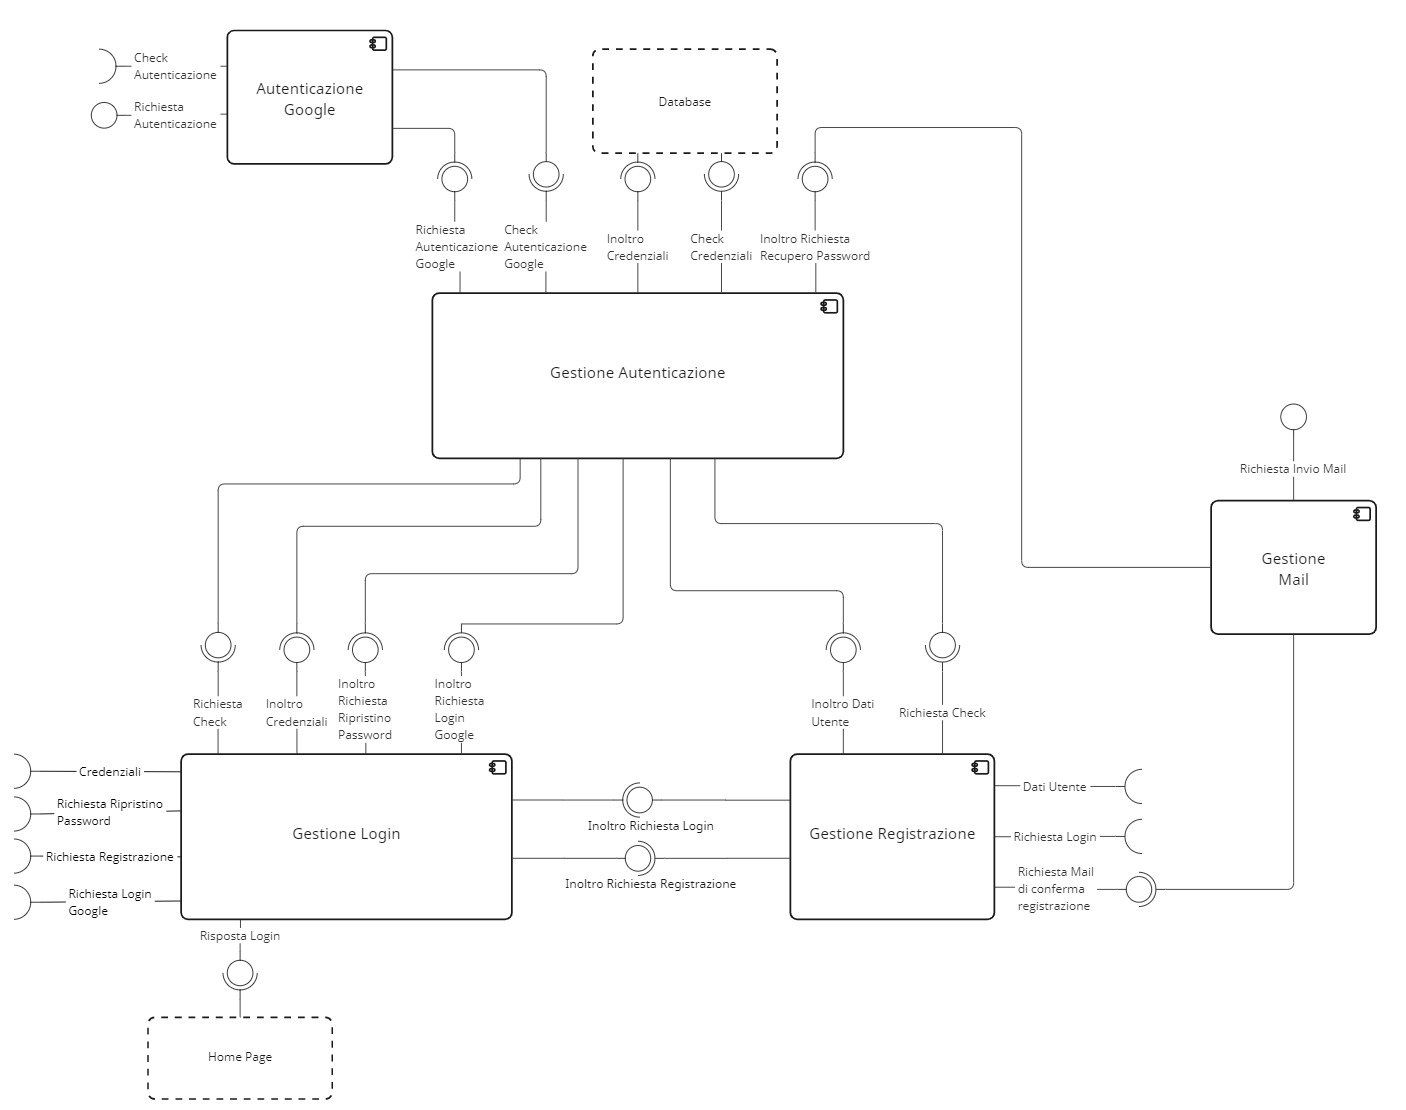
\includegraphics[width=19cm]{LoginRegistrazioneAutenticazione.jpg}
  \captionof{figure}{Component diagram Login, Registrazione, Autenticazione }
\end{center}

\section*{1 - Gestione Login}
\subsubsection*{Descrizione}
Questo componente permette di interfacciarsi direttamente con l’utente che desidera effettuare il login con le proprie credenziali. In particolare, verranno raccolti i dati dell’utente (credenziali) o eventuali richieste (recupero password) e inoltrati ad altri componenti interni per elaborarli.

\subsubsection*{Interfacce richieste}
\begin{itemize} \setlength\itemsep{0.01em}
\item {\sffamily Credenziali}: il componente riceve dall'utente username (o email) e password per accedere all'account.
\item {\sffamily Richiesta check}: il componente riceve dal componente 'Gestione autenticazione' l'esito del controllo della correttezza delle credenziali inserite dall'utente.
\item {\sffamily Richiesta ripristino password}: il componente riceve dall'utente la richiesta di ripristino della password.
\item {\sffamily Richiesta login Google}: il componente riceve dall'utente la richiesta di effettuare l'autenticazione con Google.
\item {\sffamily Richiesta registrazione}: il componente riceve dall'utente la richiesta di registrarsi e creare un nuovo account perchè non dispone ancora delle credenziali per effettuare il login.
\item {\sffamily Inoltro richiesta login}: il componente riceve la richiesta di effettuare il login dal componente 'Gestione registrazione'.
\end{itemize}

\subsubsection*{Interfacce fornite}
\begin{itemize} \setlength\itemsep{0.01em}
\item {\sffamily Risposta login}: il componente restituisce l'esito dell'operazione di autenticazione, se positivo permetterà la visualizzazione della home page tramite il componente 'Home Page' .
\item {\sffamily Inoltro richiesta registrazione}: il componente fornisce al componente 'Gestione registrazione' la richiesta di effettuare una nuova registrazione .
\item {\sffamily Inoltro credenziali}: il componente fornisce al componente 'Gestione autenticazione' le credenziali ricevute dall'utente per effettuarne i controlli.
\item {\sffamily Richiesta ripristino password}: il componente fornisce al componente 'Gestione autenticazione' la richiesta dell'utente di ripristinare la password.
\item {\sffamily Inoltro richiesta login Google}: il componente dornisce al componente 'Gestione autenticazione' la richiesta dell'utente di effettuare il login con Google.
\end{itemize}





\section*{2 - Gestione registrazione}
\subsubsection*{Descrizione}
Questo componente permette di interfacciarsi con l’utente per permettere la registrazione al sistema e la creazione di un nuovo account. I dati raccolti verranno smistati agli altri componenti che li elaboreranno.

\subsubsection*{Interfacce richieste}
\begin{itemize} \setlength\itemsep{0.01em}
\item {\sffamily Dati utente}: il componente, per permettere all'utente di registrarsi, richiede l'inserimento di nome, cognome, username, email e la password (ripetuta due volte).
\item {\sffamily Richiesta registrazione}: il componente riceve dal componente 'Gestione login' la richiesta dell'utente di effettuare la registrazione.
\item {\sffamily Richiesta check}: il componente riceve dal componente 'Gestione autenticazione' l'esito del controllo sui dati inseriti dall'utente.
\item {\sffamily Richiesta login}: il componente riceve dall'utente la richiesta di effettuare il login.
\end{itemize}

\subsubsection*{Interfacce fornite}
\begin{itemize} \setlength\itemsep{0.01em}
\item {\sffamily Richiesta mail conferma registrazione}: il componente fornisce al componente 'Gestione mail' la richiesta di inviare una mail all'utente per confermare l'avvenuta registrazione.
\item {\sffamily Inoltro richiesta login}: il componente fornisce al componente 'Gestione login' la richiesta dell'utente di effettuare il login.
\item {\sffamily Inoltro dati utente}: il componente fornisce al componente 'Gestione autenticazione' i dati inseriti dall'utente affinche essi vengano verificati.
\end{itemize}



\section*{3 - Gestione autenticazione}
\subsubsection*{Descrizione}
Questo componente è il responsabile della verifica dei dati inviati (dati di login o registrazione) e quindi dell’autenticazione degli utenti al sistema, oltre che dell'aggiornamento del database in caso di nuove registrazioni e la disconnessione dell'utente quando richiesto.
\subsubsection*{Interfacce richieste}
\begin{itemize} \setlength\itemsep{0.01em}
\item {\sffamily Inoltro dati utente}: il componente riceve dal componente 'Gestione registrazione' i dati inseriti dall'utente in fase di registrazione.
\item {\sffamily Inoltro credenziali}: il componente riceve dal componente 'Gestione login' i dati inseriti dall'utente in fase di login (le credenziali).
\item {\sffamily Richiesta ripristino password}: il componente riceve dal componente 'Gestione login' la richiesta dell'utente di recuperare la password.
\item {\sffamily Richiesta login Google}: il componente riceve dal componente 'Gestione login' la richiesta dell'utente di effettuare il login con google invece che con le credenziali.
\item {\sffamily Check credenziali}: il componente riceve dal componente 'Database' le informazioni per effettuare il controllo sulle credenziali inserite, in modo da permettere o negare l'autenticazione.
\item {\sffamily Check autenticazione Google}: il componente riceve dal componente 'Autenticazione Google' l'esito dell'autenticazione con Google.
\item {\sffamily Richiesta disconnessione}: il componente riceve dal componente 'Gestione impostazioni' la richiesta di disconnettere l'utente dal sistema.
\end{itemize}

\subsubsection*{Interfacce fornite}
\begin{itemize} \setlength\itemsep{0.01em}
\item {\sffamily Risposta check}: il componente fornisce al componente 'Gestione registrazione' l'esito del check sui dati inseriti dall'utente.
\item {\sffamily Richiesta check}:  il componente fornisce al componente 'Gestione login' l'esito del check sulle credenziali inserite dall'utente..
\item {\sffamily Inoltro richiesta ripristino password}: il componente fornisce al componente 'Gestione mail' la richiesta di inviare una mail all'utente per permettergli di recuperare la password.
\item {\sffamily Inoltro richiesta autenticazione Google}: il componente fornisce al componente 'Autenticazione Google' la richiesta di effettuare il login con Google.
\item {\sffamily Inoltro credenziali}: il componente fornisce al componente 'Database' i dati inseriti dall'utente in fase di registrazione e le sue credenziali affinchè vengano salvate nel database.

\end{itemize}

\section*{4 -  Autenticazione  Google}
\subsubsection*{Descrizione}
Questo componente interfaccia il nostro sistema con il sistema di auteticazione di Google e permette all'utente di accedere con Google invece che con le credenziali. In particolare, gestisce le richieste di autenticazione con Google e gli esiti di tali richieste. 
\subsubsection*{Interfacce richieste}
\begin{itemize} \setlength\itemsep{0.01em}
\item {\sffamily Inoltro richiesta autenticazione Google}: il componente riceve dal componente 'Gestione autenticazione' la richiesta di autenticare l'utente tramite Google.
\item {\sffamily Check autenticazione}: il componente richiede l'esito dell'autenticazione ai servizi di Google.

\end{itemize}

\subsubsection*{Interfacce fornite}
\begin{itemize} \setlength\itemsep{0.01em}
\item {\sffamily Richiesta autenticazione}: il componente invia la richiesta di autenticazione ai servizi di Google, che si occuperanno di autenticare l'utente.
\item {\sffamily Check autenticazione Google}: il componente fornisce l'esito dell'autententicazione arrivatogli da Google al componente 'Gestione autenticazione'.
\end{itemize}



\section*{5 -  Gestione mail}
\subsubsection*{Descrizione}
Questo componente interfaccia il nostro sistema con Gmail e permette di inviare delle notifiche (email) all'utente per permettergli di recuperare la password, confermare la registrazione e notificare l'approssimarsi di un evento. 
\subsubsection*{Interfacce richieste}
\begin{itemize} \setlength\itemsep{0.01em}
\item {\sffamily Inoltro richiesta ripristino password}: il componente riceve dal componente 'Gestione autenticazione' la richiesta di inviare una mail all'utente per permettergli di ripristinare la propria password.
\item {\sffamily Richiesta mail conferma registrazione}: il componente riceve dal componente 'Gestione login' la richiesta di inviare una mail all'utente per confermare la registrazione.
\item {\sffamily Richiesta invio notifica}: il componente riceve dal componente 'Gestione eventi' la richiesta di ricevere una notifica per segnalare l'approssimarsi di un proprio evento salvato.

\end{itemize}

\subsubsection*{Interfacce fornite}
\begin{itemize} \setlength\itemsep{0.01em}
\item {\sffamily Richiesta invio mail}: il componente invia la richiesta a Gmail, che si occuperanno di inviare la mail all'utente.
\end{itemize}



\clearpage
\begin{center}
  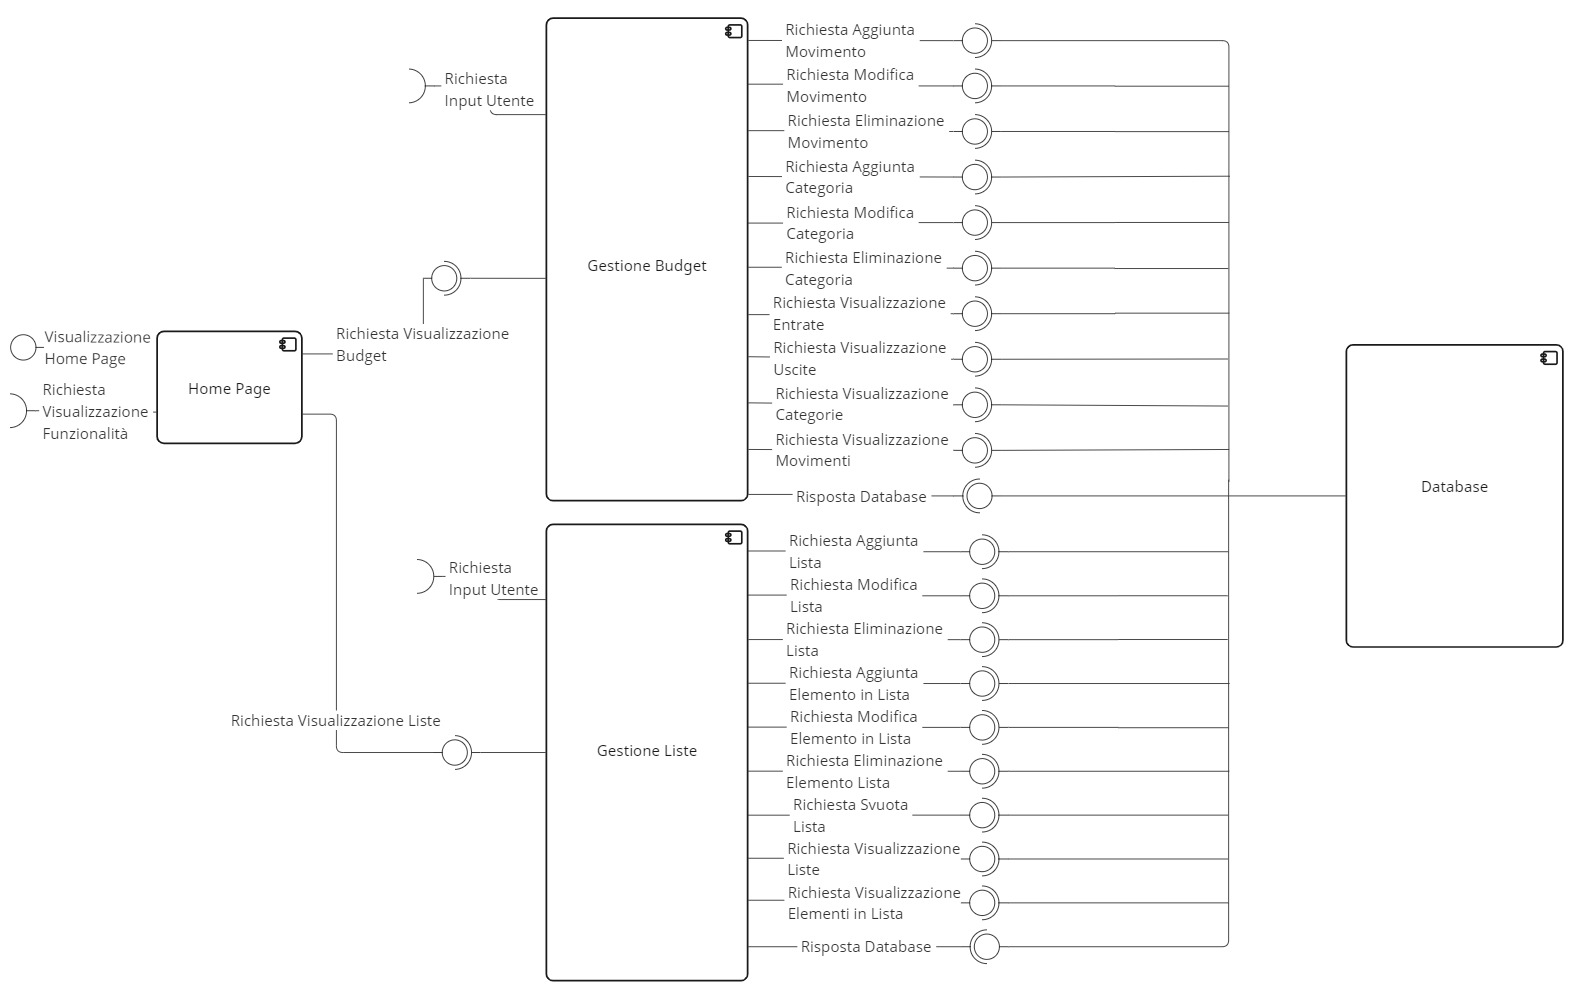
\includegraphics[width=19cm]{HomeBudgetListe.jpg}
  \captionof{figure}{Component diagram Home Page, Budget, Liste }
\end{center}

\section*{6 -  Home page}
\subsubsection*{Descrizione}
Questo componente interfaccia il nostro sistema con l'utente permettendogli, una volta effettuato il login, di visualizzare e accedere alle varie funzionalità dell'applicazione. 
\subsubsection*{Interfacce richieste}
\begin{itemize} \setlength\itemsep{0.01em}
\item {\sffamily Risposta login}: il componente richiede al componente 'Gestione login' l'esito dell'autenticazione dell'utente.
\item {\sffamily Richiesta visualizzazione funzionalità}: il componente riceve dall'utente la richiesta di accedere a una determinata funzionalità del sistema e di visualizzarne (o eventualmente poi andare a modificarne) le informazioni. Per semplicità e chiarezza questa interfaccia è unica per tutte le funzionalità, altrimenti la versione più completa (ma più confusionaria e meno leggibile) prevederebbe 8 interfacce, una per ogni funzionalità (budget, liste, eventi, mappa, ricette, carte fedeltà, impostazioni e profilo).

\end{itemize}

\subsubsection*{Interfacce fornite}
\begin{itemize} \setlength\itemsep{0.01em}
\item {\sffamily Visualizzazione home page}: il componente permette all'utente di visualizzare l'home page con tutte le funzionalità.
\item {\sffamily Richiesta visualizzazione budget}: il componente fornisce al componente 'Gestione budget' la richiesta dell'utente di accedere alla funzionalità budget e visualizzarne le informazioni.
\item {\sffamily Richiesta visualizzazione liste}: il componente fornisce al componente 'Gestione liste' la richiesta dell'utente di accedere alla funzionalità liste e visualizzarne le informazioni.
\item {\sffamily Richiesta visualizzazione eventi}: il componente fornisce al componente 'Gestione eventi' la richiesta dell'utente di accedere alla funzionalità eventi e visualizzarne le informazioni.
\item {\sffamily Richiesta visualizzazione ricette}: il componente fornisce al componente 'Gestione ricette' la richiesta dell'utente di accedere alla funzionalità ricette e visualizzarne le informazioni.
\item {\sffamily Richiesta visualizzazione mappa}: il componente fornisce al componente 'Gestione mappa' la richiesta dell'utente di accedere alla funzionalità mappa e visualizzarne le informazioni.
\item {\sffamily Richiesta visualizzazione carte fedeltà}: il componente fornisce al componente 'Gestione carte fedeltà' la richiesta dell'utente di accedere alla funzionalità carte fedeltà e visualizzarne le informazioni.
\item {\sffamily Richiesta visualizzazione profilo}: il componente fornisce al componente 'Gestione profilo' la richiesta dell'utente di accedere alla funzionalità relativa al profilo e visualizzarne le informazioni.
\item {\sffamily Richiesta visualizzazione impostazioni}: il componente fornisce al componente 'Gestione impostazioni' la richiesta dell'utente di accedere alla funzionalità relativa alle impostazioni e visualizzarne le informazioni.
\end{itemize}





\section*{7 -  Gestione budget}
\subsubsection*{Descrizione}
Questo componente è responsabile di tutti gli aspetti relativi alla funzionalità budget e in base alle richieste dell'utente permette la visualizzazione, gestione, aggiunta e rimozione del proprio budget e dei propri movimenti.
\subsubsection*{Interfacce richieste}
\begin{itemize} \setlength\itemsep{0.01em}
\item {\sffamily Richiesta visualizzazione budget}: il componente riceve dal componente 'Home page'  la richiesta di accedere alla funzionalità budget e di visualizzare il proprio budget e i propri movimenti (sia complessivamente che classificati per categoria, oppure visualizzare solo le entrate o le uscite).
\item {\sffamily Richiesta input utente}: il componente riceve dall'utente la richiesta di aggiungere, rimuovere o modificare i propri movimenti. Inoltre questa interfaccia si occupa di richiedere all'utente di inserire i dati relativi ai movimenti che intende aggiungere o modificare).
\item {\sffamily Risposta database}: il componente riceve dal componente 'Database' le informazioni che riguardano il budget e i movimenti (in base a quanto richiesto al database tramite le interfacce fornite).
\end{itemize}

\subsubsection*{Interfacce fornite}
\begin{itemize} \setlength\itemsep{0.01em}
\item {\sffamily Richiesta aggiunta movimento}: il componente fornisce al componente 'Database' la richiesta dell'utente di inserire un nuovo movimento, insieme ai dati inseriti dall'utente legati al nuovo movimento, affichè vengano scritti sul database creando tale nuovo movimento.
\item {\sffamily Richiesta modifica movimento}: il componente fornisce al componente 'Database'  la richiesta dell'utente di modificare un movimento esistente, insieme ai dati inseriti dall'utente legati a tale modifica, affichè vengano scritti sul database modificando tale movimento.
\item {\sffamily Richiesta eliminazione movimento}: il componente fornisce al componente 'Database'  la richiesta dell'utente di eliminare un movimento esistente.
\item {\sffamily Richiesta aggiunta categoria}: il componente fornisce al componente 'Database' la richiesta dell'utente di aggiungere una nuova categoria di movimento, insieme ai dati inseriti dall'utente relativi a tale categoria.
\item {\sffamily Richiesta modifica categoria}: il componente fornisce al componente 'Database' la richiesta dell'utente di modificare una categoria di movimento esistente, insieme ai dati inseriti dall'utente relativi a tale categoria.
\item {\sffamily Richiesta eliminazione categoria}: il componente fornisce al componente 'Database' la richiesta dell'utente di eliminare una categoria di movimento esistente.
\item {\sffamily Richiesta visualizzazione movimenti}: il componente fornisce al componente 'Database' una richiesta per ottenere i dati relativi al budget (tutti i movimenti).
\item {\sffamily Richiesta visualizzazione entrate}: il componente fornisce al componente 'Database' una richiesta per ottenere i dati relativi ai soli movimenti in entrata.
\item {\sffamily Richiesta visualizzazione uscite}: il componente fornisce al componente 'Database' una richiesta per ottenere i dati relativi ai soli movimenti in uscita.
\item {\sffamily Richiesta visualizzazione categoria}: il componente fornisce al componente 'Database' una richiesta per ottenere i dati relativi alla categoria di movimento richiesta dall'utente.
\end{itemize}


\section*{8 -  Gestione liste}
\subsubsection*{Descrizione}
Questo componente è responsabile di tutti gli aspetti relativi alla funzionalità liste e in base alle richieste dell'utente permette la visualizzazione, gestione, aggiunta e rimozione delle proprie liste di interesse.
\subsubsection*{Interfacce richieste}
\begin{itemize} \setlength\itemsep{0.01em}
\item {\sffamily Richiesta visualizzazione liste}: il componente riceve dal componente 'Home page'  la richiesta di accedere alla funzionalità liste e di visualizzarne le informazioni.
\item {\sffamily Richiesta input utente}: il componente riceve dall'utente la richiesta di aggiungere, rimuovere o modificare le proprie liste (e gli elementi all'interno delle liste). Inoltre questa interfaccia si occupa di richiedere all'utente di inserire i dati relativi a liste o elementi che intende aggiungere o modificare).
\item {\sffamily Risposta database}: il componente riceve dal componente 'Database' le informazioni che riguardano le liste (in base a quanto richiesto al database tramite le interfacce fornite).
\item {\sffamily Richiesta aggiunta ingredienti a lista spesa}: il componente riceve dal componente 'Gestione ricette' la richiesta di aggiungere elementi (che corrispondono agli ingredienti della ricetta) alla lista della spesa.

\end{itemize}

\subsubsection*{Interfacce fornite}
\begin{itemize} \setlength\itemsep{0.01em}
\item {\sffamily Richiesta aggiunta lista}: il componente fornisce al componente 'Database' la richiesta dell'utente di inserire una nuova lista, insieme ai dati inseriti dall'utente legati alla nuova lista, affichè vengano scritti sul database creando tale nuova lista.
\item {\sffamily Richiesta modifica lista}: il componente fornisce al componente 'Database'  la richiesta dell'utente di modificare una lista esistente, insieme ai dati inseriti dall'utente legati a tale modifica, affichè vengano scritti sul database modificando tale lista.
\item {\sffamily Richiesta eliminazione lista}: il componente fornisce al componente 'Database'  la richiesta dell'utente di eliminare una lista esistente.
\item {\sffamily Richiesta aggiunta elemento in lista}: il componente fornisce al componente 'Database' la richiesta dell'utente di aggiungere un nuovo elemento in una lista, insieme ai dati inseriti dall'utente relativi a tale elemento.
\item {\sffamily Richiesta modifica elemento in lista}: il componente fornisce al componente 'Database' la richiesta dell'utente di modificare un elemento  esistente di una lista, insieme ai dati inseriti dall'utente relativi a tale elemento.
\item {\sffamily Richiesta eliminazione elemento in lista}: il componente fornisce al componente 'Database' la richiesta dell'utente di eliminare un elemento esistente di una lista.
\item {\sffamily Richiesta visualizzazione liste}: il componente fornisce al componente 'Database' una richiesta per ottenere e visualizzare l'elenco delle liste esistenti.
\item {\sffamily Richiesta visualizzazione elementi in lista}: il componente fornisce al componente 'Database' una richiesta per ottenere e visualizzare gli elementi di una specifica lista.
\item {\sffamily Richiesta svuota lista}: il componente fornisce al componente 'Database' una richiesta per eliminare gli elementi della lista di cui non ha più interesse.
\end{itemize}

\newpage
\begin{center}
  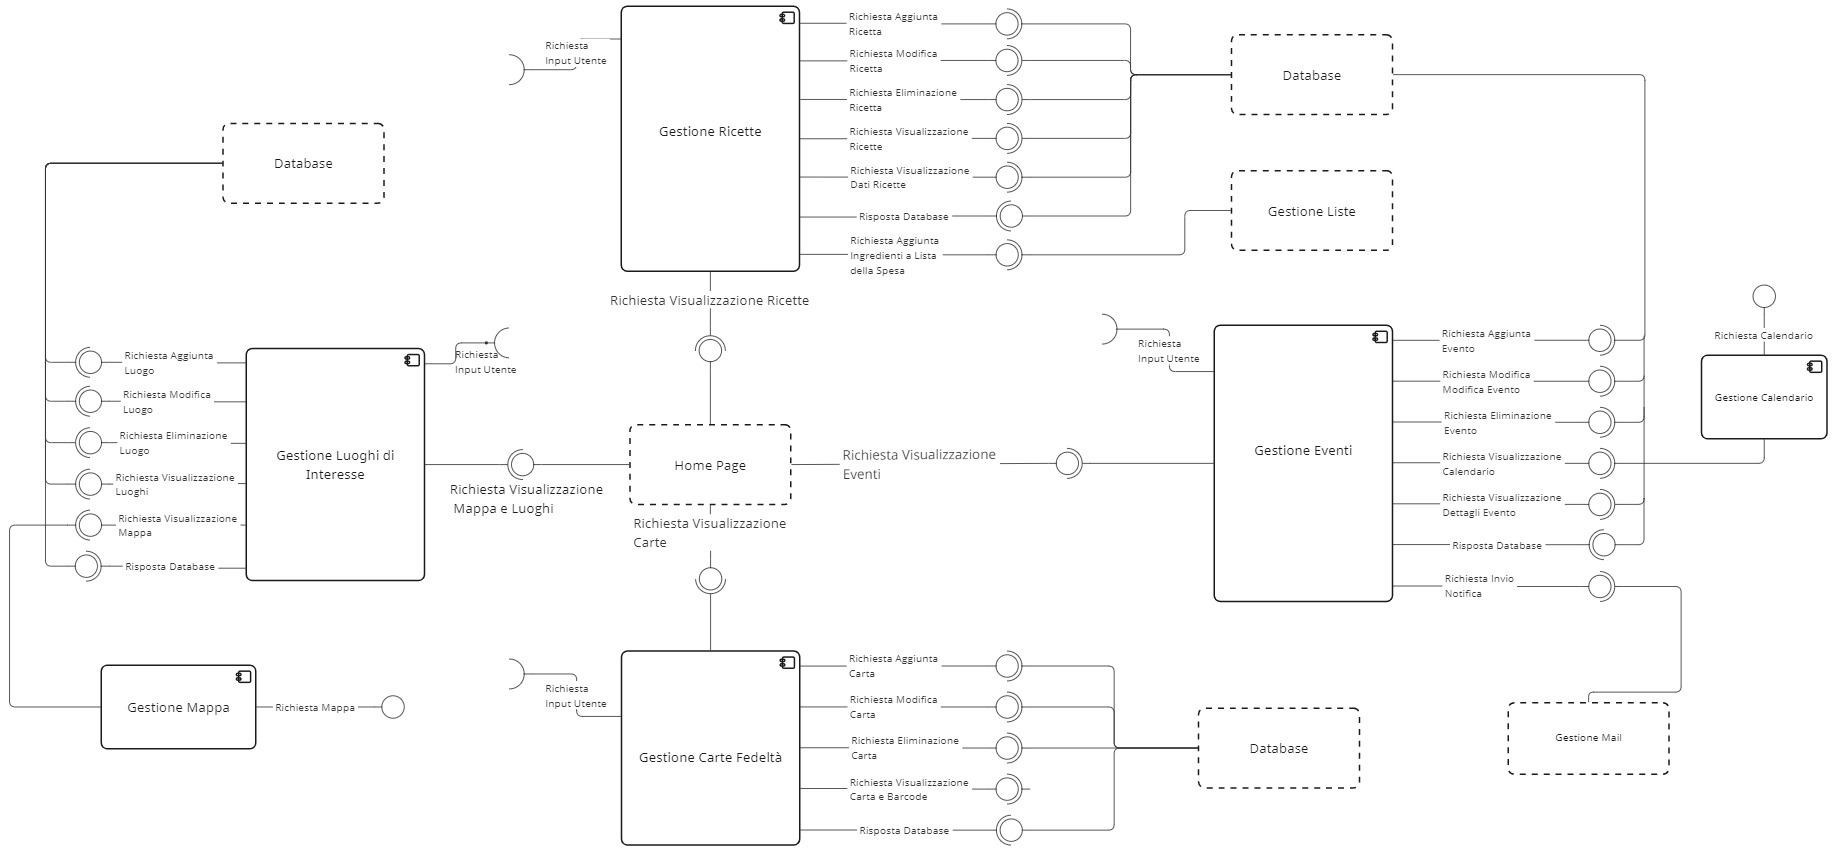
\includegraphics[width=19cm]{images/RicetteMappeEventiCarte.jpg}
  \captionof{figure}{Component diagram Ricette, Luoghi di Interesse, Eventi, Carte Fedeltà }
\end{center}

\section*{9 -  Gestione ricette}
\subsubsection*{Descrizione}
Questo componente è responsabile di tutti gli aspetti relativi alla funzionalità ricette e in base alle richieste dell'utente permette la visualizzazione, gestione, aggiunta e rimozione delle proprie ricette.
\subsubsection*{Interfacce richieste}
\begin{itemize} \setlength\itemsep{0.01em}
\item {\sffamily Richiesta visualizzazione ricette}: il componente riceve dal componente 'Home page'  la richiesta di accedere alla funzionalità ricette e di visualizzarne le informazioni.
\item {\sffamily Richiesta input utente}: il componente riceve dall'utente la richiesta di aggiungere, rimuovere o modificare le proprie ricette. Inoltre questa interfaccia si occupa di richiedere all'utente di inserire i dati relativi alla ricetta che intende aggiungere o modificare).
\item {\sffamily Risposta database}: il componente riceve dal componente 'Database' le informazioni che riguardano le ricette (in base a quanto richiesto al database tramite le interfacce fornite).

\end{itemize}

\subsubsection*{Interfacce fornite}
\begin{itemize} \setlength\itemsep{0.01em}
\item {\sffamily Richiesta aggiunta ricetta}: il componente fornisce al componente 'Database' la richiesta dell'utente di inserire una nuova ricetta, insieme ai dati inseriti dall'utente legati alla nuova ricetta, affichè vengano scritti sul database creando tale nuova ricetta.
\item {\sffamily Richiesta modifica ricetta}: il componente fornisce al componente 'Database'  la richiesta dell'utente di modificare una ricetta esistente, insieme ai dati inseriti dall'utente legati a tale modifica, affichè vengano scritti sul database modificando tale ricetta.
\item {\sffamily Richiesta eliminazione ricetta}: il componente fornisce al componente 'Database'  la richiesta dell'utente di eliminare una ricetta esistente.
\item {\sffamily Richiesta aggiunta ingredienti a lista spesa}: il componente fornisce al componente 'Database' una richiesta per inserire gli ingredienti che compongono la ricetta direttamente nella lista della spesa.
\item {\sffamily Richiesta visualizzazione ricette}: il componente fornisce al componente 'Database' una richiesta per ottenere e visualizzare l'elenco delle ricette esistenti.
\item {\sffamily Richiesta visualizzazione dati ricetta}: il componente fornisce al componente 'Database' una richiesta per ottenere e visualizzare i dati relativi ad una specifica ricetta.
\item {\sffamily Richiesta aggiunta ingredienti a lista spesa}:il componente fornisce al componente 'Gestione liste' la richiesta di inserire tutti o alcuni ingredienti alla lista della spesa.
\end{itemize}



\section*{10 -  Gestione eventi}
\subsubsection*{Descrizione}
Questo componente è responsabile di tutti gli aspetti relativi alla funzionalità eventi e in base alle richieste dell'utente permette la visualizzazione, gestione, aggiunta e rimozione dei propri eventi/attività.
\subsubsection*{Interfacce richieste}
\begin{itemize} \setlength\itemsep{0.01em}
\item {\sffamily Richiesta visualizzazione eventi}: il componente riceve dal componente 'Home page'  la richiesta di accedere alla funzionalità eventi e di visualizzarne le informazioni.
\item {\sffamily Richiesta input utente}: il componente riceve dall'utente la richiesta di aggiungere, rimuovere o modificare i propri eventi. Inoltre questa interfaccia si occupa di richiedere all'utente di inserire i dati relativi agli eventi che intende aggiungere o modificare).
\item {\sffamily Risposta database}: il componente riceve dal componente 'Database' le informazioni che riguardano gli eventi (in base a quanto richiesto al database tramite le interfacce fornite).

\end{itemize}

\subsubsection*{Interfacce fornite}
\begin{itemize} \setlength\itemsep{0.01em}
\item {\sffamily Richiesta aggiunta evento}: il componente fornisce al componente 'Database' la richiesta dell'utente di inserire un nuovo evento, insieme ai dati inseriti dall'utente legati al nuovo evento, affichè vengano scritti sul database creando tale nuovo evento.
\item {\sffamily Richiesta modifica evento}: il componente fornisce al componente 'Database'  la richiesta dell'utente di modificare un evento esistente, insieme ai dati inseriti dall'utente legati a tale modifica, affichè vengano scritti sul database modificando tale evento.
\item {\sffamily Richiesta eliminazione evento}: il componente fornisce al componente 'Database'  la richiesta dell'utente di eliminare un evento esistente.
\item {\sffamily Richiesta visualizzazione calendario}: il componente fornisce al componente 'Gestione calendario' una richiesta visualizzare il calendario con segnati gli eventi salvati dall'utente.
\item {\sffamily Richiesta visualizzazione dettagli evento}: il componente fornisce al componente 'Database' una richiesta per ottenere e visualizzare i dati relativi ad un specifico evento.
\item {\sffamily Richiesta invio notifica}: il componente fornisce al componente 'Gestione mail' la richiesta di inviare una email all'utente per segnalare l'approssimarsi di un evento/attività di cui esso vuole essere ricordato.
\end{itemize}




\section*{11 -  Gestione mappe/luoghi di interesse}
\subsubsection*{Descrizione}
Questo componente è responsabile di tutti gli aspetti relativi alla funzionalità mappe/luoghi di interesse e in base alle richieste dell'utente permette la visualizzazione, gestione, aggiunta e rimozione dei propri luoghi di interesse.
\subsubsection*{Interfacce richieste}
\begin{itemize} \setlength\itemsep{0.01em}
\item {\sffamily Richiesta visualizzazione mappa e luoghi}: il componente riceve dal componente 'Home page'  la richiesta di accedere alla funzionalità mappa e di visualizzare le informazioni relative ai luoghi di interesse.
\item {\sffamily Richiesta input utente}: il componente riceve dall'utente la richiesta di aggiungere, rimuovere o modificare i propri luoghi di interesse. Inoltre questa interfaccia si occupa di richiedere all'utente di inserire i dati relativi ai luoghi che intende aggiungere o modificare).
\item {\sffamily Risposta database}: il componente riceve dal componente 'Database' le informazioni che riguardano i luoghi di interesse (in base a quanto richiesto al database tramite le interfacce fornite).

\end{itemize}

\subsubsection*{Interfacce fornite}
\begin{itemize} \setlength\itemsep{0.01em}
\item {\sffamily Richiesta aggiunta luogo}: il componente fornisce al componente 'Database' la richiesta dell'utente di inserire un nuovo luogo di interesse, insieme ai dati inseriti dall'utente legati al nuovo luogo, affichè vengano scritti sul database creando tale nuovo luogo.
\item {\sffamily Richiesta modifica luogo}: il componente fornisce al componente 'Database'  la richiesta dell'utente di modificare un luogo di interesse esistente, insieme ai dati inseriti dall'utente legati a tale modifica, affichè vengano scritti sul database modificando tale luogo.
\item {\sffamily Richiesta eliminazione luogo}: il componente fornisce al componente 'Database' la richiesta dell'utente di eliminare un luogo di interesse esistente.
\item {\sffamily Richiesta visualizzazione mappa}: il componente fornisce al componente 'Gestione mappa' una richiesta visualizzare la mappa con segnati i luoghi di interesse salvati dall'utente.
\item {\sffamily Richiesta visualizzazione dettagli luogo}: il componente fornisce al componente 'Database' una richiesta per ottenere e visualizzare i dati relativi ad un specifico luogo.
\end{itemize}



\section*{12 -  Gestione carte fedeltà}
\subsubsection*{Descrizione}
Questo componente è responsabile di tutti gli aspetti relativi alla funzionalità carte fedeltà e in base alle richieste dell'utente permette la visualizzazione, gestione, aggiunta e rimozione delle proprie carte fedeltà.
\subsubsection*{Interfacce richieste}
\begin{itemize} \setlength\itemsep{0.01em}
\item {\sffamily Richiesta visualizzazione carte}: il componente riceve dal componente 'Home page'  la richiesta di accedere alla funzionalità carte fedeltà e di visualizzare le informazioni relative alle carte.
\item {\sffamily Richiesta input utente}: il componente riceve dall'utente la richiesta di aggiungere, rimuovere o modificare le proprie carte fedeltà. Inoltre questa interfaccia si occupa di richiedere all'utente di inserire i dati relativi alla carta fedeltà che intende aggiungere o modificare).
\item {\sffamily Risposta database}: il componente riceve dal componente 'Database' le informazioni che riguardano i luoghi di interesse (in base a quanto richiesto al database tramite le interfacce fornite).

\end{itemize}

\subsubsection*{Interfacce fornite}
\begin{itemize} \setlength\itemsep{0.01em}
\item {\sffamily Richiesta aggiunta carta}: il componente fornisce al componente 'Database' la richiesta dell'utente di inserire una nuova carta fedeltà, insieme ai dati inseriti dall'utente legati alla nuova carta, affichè vengano scritti sul database creando tale carta.
\item {\sffamily Richiesta modifica carta}: il componente fornisce al componente 'Database'  la richiesta dell'utente di modificare una carta fedeltà esistente, insieme ai dati inseriti dall'utente legati a tale modifica, affichè vengano scritti sul database modificando tale carta.
\item {\sffamily Richiesta eliminazione carta}: il componente fornisce al componente 'Database'  la richiesta dell'utente di eliminare una carta fedeltà esistente.
\item {\sffamily Richiesta visualizzazione carta e barcode}: il componente fornisce al componente 'Database' una richiesta per ottenere e visualizzare i dati relativi ad una specifica carta (compreso il barcode generato a partire dal numero della carta).
\end{itemize}



\section*{13 -  Gestione mappa}
\subsubsection*{Descrizione}
Questo componente interfaccia il nostro sistema con OpenStreetMap per permettere la visualizzazione della mappa su cui segnalare i luoghi di interesse salvati dall'utente.
\subsubsection*{Interfacce richieste}
\begin{itemize} \setlength\itemsep{0.01em}
\item {\sffamily Richiesta visualizzazione mappa}: il componente riceve dal componente 'Gestione luoghi di interesse' la richiesta visualizzare la mappa.
\end{itemize}
\subsubsection*{Interfacce fornite}
\begin{itemize} \setlength\itemsep{0.01em}
\item {\sffamily Richiesta mappa}: il componente fornisce la richiesta a OpenStreetMap, che si occuperà di visualizzare la mappa.
\end{itemize}

\section*{14 -  Gestione calendario}
\subsubsection*{Descrizione}
Questo componente interfaccia il nostro sistema con Google Calendar per permettere la visualizzazione del calendario con gli eventi salvati dall'utente.
\subsubsection*{Interfacce richieste}
\begin{itemize} \setlength\itemsep{0.01em}
\item {\sffamily Richiesta visualizzazione calendario}: il componente riceve dal componente 'Gestione eventi' la richiesta visualizzare il calendario.
\end{itemize}
\subsubsection*{Interfacce fornite}
\begin{itemize} \setlength\itemsep{0.01em}
\item {\sffamily Richiesta mappa}: il componente fornisce la richiesta a Google Calendar, che si occuperà di visualizzare il calendario.
\end{itemize}

\newpage
\begin{center}
  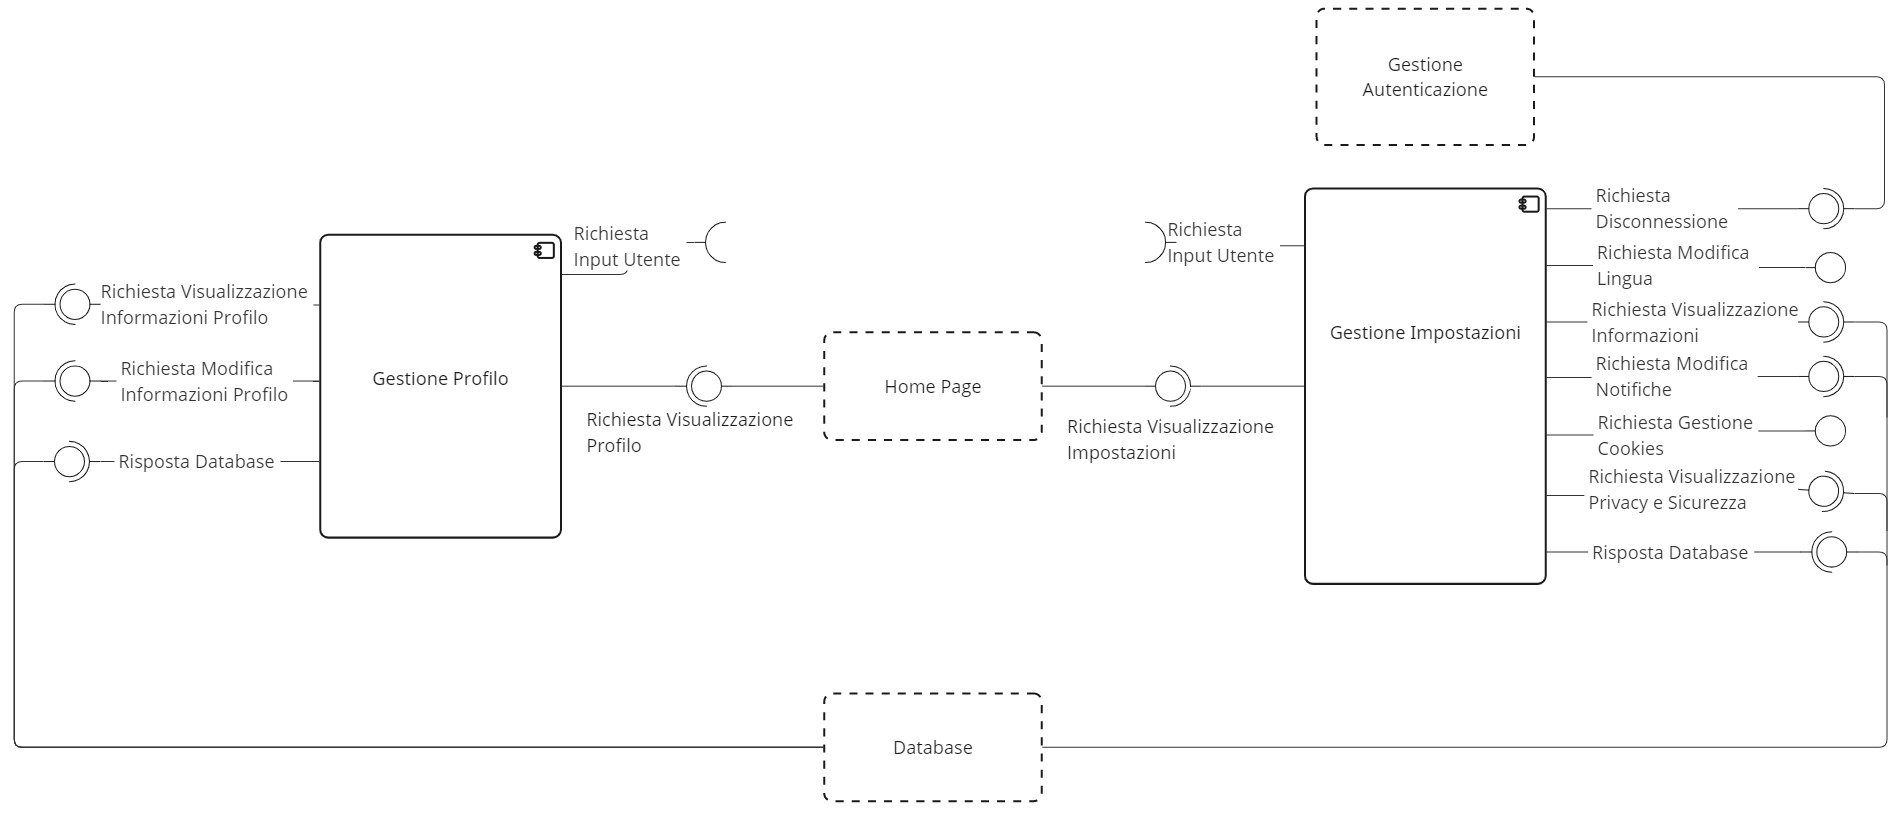
\includegraphics[width=19cm]{images/ProfiloImpostazioni.jpg}
  \captionof{figure}{Component diagram Profilo, Impostazioni}
\end{center}


\section*{15 -  Gestione Profilo}
\subsubsection*{Descrizione}
Questo componente è responsabile di tutti gli aspetti relativi alla funzionalità del profilo e in base alle richieste dell'utente permette la visualizzazione e gestione delle informazioni relative al profilo.
\subsubsection*{Interfacce richieste}
\begin{itemize} \setlength\itemsep{0.01em}
\item {\sffamily Richiesta visualizzazione profilo}: il componente riceve dal componente 'Home page'  la richiesta di accedere alla sezione profilo e di visualizzare le informazioni relative al proprio profilo.
\item {\sffamily Richiesta input utente}:  il componente, per permettere all'utente di modificare le informazioni associate il proprio profilo, richiede l'inserimento di uno o più dati relativi al profilo (nome, cognome, username, email, password).
\item {\sffamily Risposta database}: il componente riceve dal componente 'Database' le informazioni che riguardano il profilo (in base a quanto richiesto al database tramite le interfacce fornite).

\end{itemize}

\subsubsection*{Interfacce fornite}
\begin{itemize} \setlength\itemsep{0.01em}
\item {\sffamily Richiesta visualizzazione informazioni profilo}: il componente fornisce al componente 'Database'  la richiesta di visualizzare e quindi ricevere le informazioni relative al proprio profilo.
\item {\sffamily Richiesta modifica informazioni profilo}: il componente fornisce al componente 'Database' la richiesta di modificare le informazioni ruguardanti il proprio profilo (nome, cognome, username, email, password).

\end{itemize}


\section*{16 -  Gestione impostazioni}
\subsubsection*{Descrizione}
Questo componente è responsabile di tutti gli aspetti relativi alle impostazioni del sistema e in base alle richieste dell'utente permette la visualizzazione e gestione delle informazioni relative alle impostazioni.
\subsubsection*{Interfacce richieste}
\begin{itemize} \setlength\itemsep{0.01em}
\item {\sffamily Richiesta visualizzazione impostazioni}: il componente riceve dal componente 'Home page'  la richiesta di accedere alla sezione impostazioni e di visualizzare le preferenze relative alle impostazioni.
\item {\sffamily Richiesta input utente}:  il componente, per permettere all'utente di modificare le preferenze riguardo le impostazioni del sistema, richiede di inserire le proprie modifiche o preferenze  riguardanti notifiche (attive o meno), lingua, cookies.
\item {\sffamily Risposta database}: il componente riceve dal componente 'Database' le informazioni che riguardano le impostazioni (in base a quanto richiesto al database tramite le interfacce fornite).

\end{itemize}

\subsubsection*{Interfacce fornite}
\begin{itemize} \setlength\itemsep{0.01em}
\item {\sffamily Richiesta disconnessione}: il componente fornisce al componente 'Gestione autenticazione' la richiesta dell'utente disconnettersi dal sistema.
\item {\sffamily Richiesta modifica lingua}: il componente fornisce la richiesta dell'utente di modificare la lingua con cui sono visualizzate tutte le funzionalità e i dati del sistema.
\item {\sffamily Richiesta visualizzazione informazioni}: il componente fornisce al componente 'Database'  la richiesta dell'utente di visualizzare le informazioni del sistema e i contatti degli sviluppatori.
\item {\sffamily Richiesta modifica notifiche}: il componente fornisce al componente 'Database' una richiesta per attivare/disattivare l'invio di notifiche da parte del sistema verso l'utente.
\item {\sffamily Richiesta gestione cookies}: il componente fornisce una richiesta per permettere all'utente di salvare le proprie preferenze riguardanti i cookies.
\item {\sffamily Richiesta visualizzazione privacy e sicurezza}: il componente fornisce al componente 'Database' una richiesta per visualizzare le informazioni riguardanti l'informativa sulla privacy e il trattamento dei dati personali.

\end{itemize}



\section*{17 - Database}
\subsubsection*{Descrizione}
Questo componente è responsabile dell'interfacciamento con il database e permette di effettuare richieste per leggere dal  database (ottenere dati che verranno visualizzati dal sistema) oppure per scriverci (modifcarne le informazioni in base alla richieste dell'utente al sistema).
\subsubsection*{Interfacce richieste}
\begin{itemize} \setlength\itemsep{0.01em}
\item {\sffamily Inoltro dati utente/credenziali}: il componente riceve dal componente 'Gestione autenticazione' la richiesta di scrivere le credenziali e i dati inseriti dall'utente in fase di registrazione nel database.
\item {\sffamily Richiesta aggiunta movimento}: il componente riceve dal componente 'Gestione budget' la richiesta di aggiungere un nuovo movimento al database con in dati inseriti dall'utente. 
\item {\sffamily Richiesta modifica movimento}: il componente riceve dal componente 'Gestione budget' la richiesta di modificare un movimento esistente nel database con in dati inseriti dall'utente. 
\item {\sffamily Richiesta eliminazione movimento}:  il componente riceve dal componente 'Gestione budget' la richiesta di eliminare un movimento dal database.
\item {\sffamily Richiesta aggiunta categoria}:  il componente riceve dal componente 'Gestione budget' la richiesta di aggiungere una nuova categoria di movimenti al database con in dati inseriti dall'utente. 
\item {\sffamily Richiesta modifica categoria}: il componente riceve dal componente 'Gestione budget' la richiesta di modificare una categoria di movimenti esistente nel database con in dati inseriti dall'utente.
\item {\sffamily Richiesta eliminazione categoria}: il componente riceve dal componente 'Gestione budget' la richiesta di eliminare una categoria di movimenti dal database.
\item {\sffamily Richiesta visualizzazione entrate}: il componente riceve dal componente 'Gestione budget' la richiesta di ottenere i dati relativi ai soli movimenti in entrata affinchè possano essere visualizzati.  
\item {\sffamily Richiesta visualizzazione uscite}: il componente riceve dal componente 'Gestione budget' la richiesta di ottenere i dati relativi ai soli movimenti in uscita affinchè possano essere visualizzati
\item {\sffamily Richiesta visualizzazione categorie}: il componente riceve dal componente 'Gestione budget' la richiesta di ottenere i dati relativi ai movimenti riguardanti una specifica categoria affinchè possano essere visualizzati.
\item {\sffamily Richiesta visualizzazione movimenti}: il componente riceve dal componente 'Gestione budget' la richiesta di ottenere i dati relativi a tutti i movimenti affinchè possano essere visualizzati.
\item {\sffamily Richiesta aggiunta lista}: il componente riceve dal componente 'Gestione liste' la richiesta di aggiungere una nuova lista al database con in dati inseriti dall'utente.
\item {\sffamily Richiesta modifica lista}: il componente riceve dal componente 'Gestione liste' la richiesta di modificare una lista esistente nel database con in dati inseriti dall'utente.
\item {\sffamily Richiesta eliminazione lista}: il componente riceve dal componente 'Gestione liste' la richiesta di eliminare una lista dal database.
\item {\sffamily Richiesta aggiunta elemento lista}: il componente riceve dal componente 'Gestione liste' la richiesta di aggiungere un nuovo elemento ad una lista con in dati inseriti dall'utente.
\item {\sffamily Richiesta modifica elemento lista}: il componente riceve dal componente 'Gestione liste' la richiesta di modificare un elemento esistente in una lista con in dati inseriti dall'utente.
\item {\sffamily Richiesta eliminazione elemento lista}: il componente riceve dal componente 'Gestione liste' la richiesta di eliminare un elemento di una lista.
\item {\sffamily Richiesta svuota lista}: il componente riceve dal componente 'Gestione liste' la richiesta di rimuovere tutti gli elementi della lista che sono contrassegnati (cioè che non servono più all'utente).
\item {\sffamily Richiesta visualizzazione liste}: il componente riceve dal componente 'Gestione liste' la richiesta di ottenere l'elenco delle liste esistenti affinchè possano essere visualizzate.
\item {\sffamily Richiesta visualizzazione elementi in lista}: il componente riceve dal componente 'Gestione liste' la richiesta di ottenere i dati relativi agli elementi di una specifica lista affinchè possano essere visualizzati.
\item {\sffamily Richiesta aggiunta ricetta}: il componente riceve dal componente 'Gestione ricette' la richiesta di aggiungere una nuova ricetta al database con in dati inseriti dall'utente.
\item {\sffamily Richiesta modifica ricetta}: il componente riceve dal componente 'Gestione ricette' la richiesta di modificare una ricetta esistente nel database con in dati inseriti dall'utente.
\item {\sffamily Richiesta eliminazione ricetta}: il componente riceve dal componente 'Gestione ricette' la richiesta di eliminare una ricetta dal database.
\item {\sffamily Richiesta visualizzazione ricette}: il componente riceve dal componente 'Gestione ricette' la richiesta di ottenere l'elenco delle ricette esistenti affinchè possano essere visualizzate.
\item {\sffamily Richiesta visualizzazione dati ricetta}: il componente riceve dal componente 'Gestione ricette' la richiesta di ottenere i dati relativi ad una specifica ricetta affinchè possano essere visualizzati.
\item {\sffamily Richiesta aggiunta luogo}: il componente riceve dal componente 'Gestione luoghi di interesse' la richiesta di aggiungere un nuovo luogo al database con in dati inseriti dall'utente.
\item {\sffamily Richiesta modifica luogo}: il componente riceve dal componente 'Gestione luoghi di interesse' la richiesta di modificare un luogo di interesse esistente nel database con in dati inseriti dall'utente.
\item {\sffamily Richiesta eliminazione luogo}: il componente riceve dal componente 'Gestione luoghi di interesse' la richiesta di eliminare un luogo dal database.
\item {\sffamily Richiesta visualizzazione luoghi}:  il componente riceve dal componente 'Gestione luoghi di interesse' la richiesta di ottenere i dati relativi ai luoghi di interesse salvati affinchè possano essere visualizzati.
\item {\sffamily Richiesta aggiunta carta}: il componente riceve dal componente 'Gestione carte fedeltà' la richiesta di aggiungere una nuova carta fedeltà al database con in dati inseriti dall'utente.
\item {\sffamily Richiesta modifica carta}: il componente riceve dal componente 'Gestione carte fedeltà' la richiesta di modificare una carta fedeltà esistente nel database con in dati inseriti dall'utente.
\item {\sffamily Richiesta eliminazione carta}: il componente riceve dal componente 'Gestione carte fedeltà' la richiesta di eliminare una carta fedeltà dal database.
\item {\sffamily Richiesta visualizzazione carta e barcode}: il componente riceve dal componente 'Gestione carte fedeltà' la richiesta di ottenere i dati relativi ad una carta fedeltà affinchè possano essere visualizzati (con associato il barcode calcolato a partire dal numero della carta).
\item {\sffamily Richiesta aggiunta evento}:  il componente riceve dal componente 'Gestione eventi' la richiesta di aggiungere un nuovo evento al database con in dati inseriti dall'utente.
\item {\sffamily Richiesta modifica evento}: il componente riceve dal componente 'Gestione eventi' la richiesta di modificare un evento esistente nel database con in dati inseriti dall'utente.
\item {\sffamily Richiesta eliminazione evento}: il componente riceve dal componente 'Gestione eventi' la richiesta di eliminare un evento dal database.
\item {\sffamily Richiesta visualizzazione dettagli evento}: il componente riceve dal componente 'Gestione eventi' la richiesta di ottenere i dati relativi ad un evento affinchè possano essere visualizzati.
\item {\sffamily Richiesta visualizzazione informazioni profilo}: il componente riceve dal componente 'Gestione profilo' la richiesta di ottenere i dati relativi al profilo dell'utente affinchè possano essere visualizzati.
\item {\sffamily Richiesta modifica informazioni profilo}: il componente riceve dal componente 'Gestione profilo' la richiesta di modificare le informazioni relative al profilo dell'utente nel database con in dati inseriti.
\item {\sffamily Richiesta visualizzazione informazioni}: il componente riceve dal componente 'Gestione impostazioni' la richiesta di ottenere i dati relativi alle informazioni di sistema e ai contatti degli sviluppatori affinchè possano essere visualizzati.
\item {\sffamily Richiesta modifica notifiche}: il componente riceve dal componente 'Gestione impostazioni' la richiesta di modificare la preferenza dell'utente riguardo la ricezione o meno delle notifiche.
\item {\sffamily Richiesta visualizzazione privacy e sicurezza}: il componente riceve dal componente 'Gestione impostazioni' la richiesta di ottenere le informazioni relative al trattamento dei dati personali affinchè possano essere visualizzati.



\end{itemize}

\subsubsection*{Interfacce fornite}
\begin{itemize} \setlength\itemsep{0.01em}
\item {\sffamily Risposta database}: il componente fornisce ai vari componenti che hanno richiesto la lettura di dati dal database tali dati affinchè possano essere visualizzati.

\end{itemize}



\newpage
\part{Analisi delle classi}
Nel seguente capitolo analizzeremo le classi che costituiranno il sistema, andando a definire una prima architettura alle classi su cui {\scshape LifeManager} si basa, e le relazioni tra queste. 

In particolare, una classe è sostanzialmente la descrizione di un gruppo di oggetti con proprietà (attributi), comportamento (operazioni), relazioni e semantica comuni. Una relazione è una connessione tra cose (cioè classi, interfacce, componenti, package), che fornisce un pathway (strada) per la comunicazione fra oggetti.

Il risultato di questa analisi costituirà il \textit{Class Diagram}.

%immagine class diagram generale

\newpage
\section{Utente}
\begin{center}
  \includegraphics[width=4cm]{images/classutente.png}
  \captionof{figure}{Classe Utente}
\end{center}
La classe {\sffamily Utente} è la classe principale in cui vengono memorizzate tutte le informazioni relative all'utente e le impostazioni che vengono salvate. 
\subsubsection*{Attributi}
\begin{itemize} \setlength\itemsep{0.01em}
\item {\ttfamily id\_user}: valore intero che identifica univocamente l'utente nell'intero database. 
\item {\ttfamily nome}: stringa contenente il nome anagrafico dell'utente. 
\item {\ttfamily cognome}: stringa contenente il cognome anagrafico dell'utente. 
\item {\ttfamily username}: stringa contenente il nome che l'utente ha scelto per farsi identificare univocamente all'interno del sistema.
\item {\ttfamily email}: stringa contenente l'indirizzo di posta elettronica dell'utente. 
\item {\ttfamily password}: stringa contenente la password cifrata dell'utente.
\item {\ttfamily lingua}: stringa contenente la lingua che l'utente ha scelto per operare nel sistema.
\item {\ttfamily cookies}: stringa contenente valori che identificano i cookies che l'utente ha scelto di accettare o non accettare, secondo un ordine preciso. 
\end{itemize}
\subsubsection*{Metodi}
\begin{itemize} \setlength\itemsep{0.01em}
\item {\ttfamily registrazione}: metodo che viene invocato alla registrazione che comporta l'inserimento nel database dell'utente.
\item {\ttfamily conferma\_email}: metodo che viene invocato quando, dopo aver effettuato la registrazione, l'utente riceve una mail in cui attraverso un link, attiva il profilo. 
\item {\ttfamily login}: metodo che viene invocato ogni qual volta che l'utente deve effettuare il login. Attraverso questo metodoo, l'utente anonimo diviene utente autenticato.
\item {\ttfamily logout}: metodo che viene invocato quando l'utente intende uscire dall'applicazione. Con questo metodo l'utente autenticato diventa utente anonimo.
\item {\ttfamily modifica\_lingua}: metodo che viene invocato quando l'utente, che si trova nella sezione relativa alle impostazioni, desidera modificare la lingua del sistema.
\item {\ttfamily modifica\_cookies}:  metodo che viene invocato quando l'utente, che si trova nella sezione relativa alle impostazioni, desidera modificare la lista dei cookies accettati, per usufruire del sistema.
\end{itemize}
\subsubsection*{Object Constraint Language (OCL)}
\begin{itemize}
\item {\ttfamily context Utente \\inv NomeLunghezza: self.nome.size() >= 1 and self.nome.size() <= 100}
\item {\ttfamily context Utente \\inv CognomeLunghezza: self.cognome.size() >= 1 and self.cognome.size <= 100}
\item {\ttfamily context Utente \\inv UsernameLunghezza: self.username.size() >= 1 and self.username.size <= 100}
\item {\ttfamily context Utente::registrazione() \\pre self.nome->notEmpty \\pre self.cognome->notEmpty
\\pre self.username->notEmpty
\\pre self.email->notEmpty
\\pre self.password->notEmpty}
\item {\ttfamily context Utente \\inv PasswordLunghezza: self.password.size() >= 8}
\item {\ttfamily context Utente::modifica\_lingua() 
\\post self.lingua = NuovaLingua}
\item {\ttfamily context Utente::modifica\_cookies() 
\\post self.cookies = NuoviCookies}
\end{itemize}

\newpage
\section{Data}
\begin{center}
  \includegraphics[width=3cm]{images/classdata.png}
  \captionof{figure}{Classe Data}
\end{center}
La classe {\sffamily Data} è la classe in cui è mostrata la struttura di ogni data presente nel sistema. 
\subsubsection*{Attributi}
\begin{itemize} \setlength\itemsep{0.01em}
\item {\ttfamily anno}: intero contenente l'anno.
\item {\ttfamily mese}: intero contenente il mese.
\item {\ttfamily giorno}: intero contenente il giorno.
\item {\ttfamily ora}: intero contenente l'ora (formato 24 ore).
\item {\ttfamily minuti}: intero contenente i minuti.

\end{itemize}
\newpage
\begin{center}
  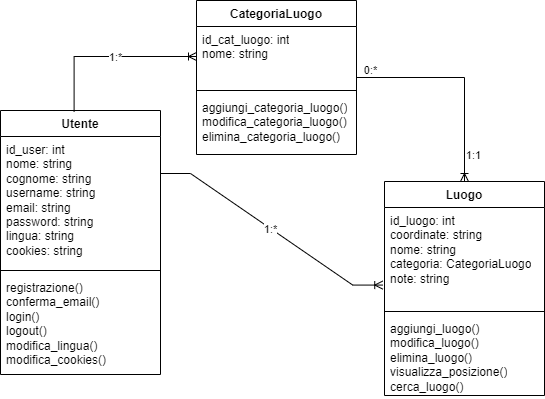
\includegraphics[width=11cm]{images/classmappe.png}
  \captionof{figure}{Classi Luogo e CategoriaLuogo}
\end{center}
\section{Categoria Luogo}
 
La classe {\sffamily CategoriaLuogo} permette di descrivere gli oggetti che rappresentano le categorie con cui l'utente classifica i propri luoghi e descrive le operazione possibili per ogni oggetto di questo tipo.

\subsubsection*{Attributi}
\begin{itemize} \setlength\itemsep{0.01em}
\item {\ttfamily id\_cat\_luogo}: intero contenente un numero progressivo che identifica la precisa categoria.
\item {\ttfamily nome}: stringa contenente il nome che l'utente sceglie di dare alla categoria.
\end{itemize}
\subsubsection*{Metodi}
\begin{itemize} \setlength\itemsep{0.01em}
\item {\ttfamily aggiungi\_categoria\_luogo}: metodo che l'utente invoca quando deve creare una nuova categoria. Il sistema, attraverso tal funzione, la inserisce nel database.
\item {\ttfamily modifica\_categoria\_luogo}: metodo che l'utente invoca quando desidera modificare il nome di una categoria.
\item {\ttfamily elimina\_categoria\_luogo}: metodo che l'utente invoca quando desidera cancellare una categoria. L'eliminazione non comporta la cancellazione dei luoghi associati alla categoria.
\end{itemize}
\subsubsection*{Object Constraint Language (OCL)}
\begin{itemize} \setlength\itemsep{0.01em}
\item {\ttfamily context CategoriaLuogo inv NomeLunghezza: self.nome.size() >= 1}
\item {\ttfamily context CategoriaLuogo::aggiungi\_categoria\_luogo() \\pre self.nome->notEmpty()}
\end{itemize}

\section{Luogo}
La classe {\sffamily Luogo} permette di descrivere gli oggetti che rappresentano i luoghi dei quali l'utente vuole tener traccia e descrive le operazione possibili per ogni oggetto di questo tipo. 
\subsubsection*{Attributi}
\begin{itemize} \setlength\itemsep{0.01em}
\item {\ttfamily id\_luogo}: intero contenente un numero progressivo che identifica il preciso luogo.
\item {\ttfamily coordinate}: stringa contenente le coordinate a cui si riferisce un luogo.
\item {\ttfamily nome}: stringa contenente il nome che l'utente desidera dare al luogo.
\item {\ttfamily categoria}: stringa contenente il nome della categoria a cui il luogo è associato
\item {\ttfamily note}: stringa contenente le note che l'utente desidera inserire.
\end{itemize}
\subsubsection*{Metodi}
\begin{itemize} \setlength\itemsep{0.01em}
\item {\ttfamily aggiungi\_luogo}: metodo che l'utente invoca quando deve inserire un nuovo luogo. Il sistema, attraverso tal funzione, lo inserisce nel database.
\item {\ttfamily modifica\_luogo}: metodo che l'utente invoca quando desidera modificare qualunque attributo del luogo.
\item {\ttfamily elimina\_luogo}: metodo che l'utente invoca quando desidera eliminare un luogo. 
\item {\ttfamily visualizza\_posizione}: metodo che l'utente invoca quando desidera visualizzare la posizione (attrzverso un segnaposto) sulla mappa.
\item {\ttfamily cerca\_luogo}: metodo che l'utente invoca quando desidera cercare un luogo. 
\end{itemize}
\subsubsection*{Object Constraint Language (OCL)}
\begin{itemize}
\item {\ttfamily context Luogo inv NomeLunghezza: self.nome.size() >= 1}
\item {\ttfamily context Luogo::aggiungi\_luogo() \\pre self.nome->notEmpty()
\\pre self.categoria->notEmpty()}

\end{itemize}
\newpage
\begin{center}
  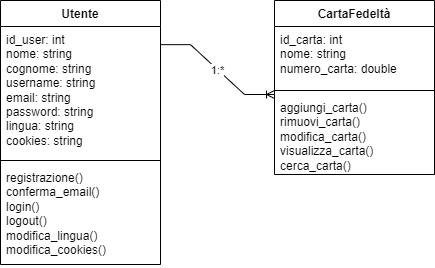
\includegraphics[width=7cm]{images/classcartefed.png}
  \captionof{figure}{Classe Carta fedeltà}
\end{center}
\section{Carta fedeltà}

La classe {\sffamily CartaFedeltà} permette di descrivere gli oggetti che rappresentano le carte fedeltà dell'utente e descrive le operazione possibili per ogni oggetto di questo tipo.
\subsubsection*{Attributi}
\begin{itemize} \setlength\itemsep{0.01em}
\item {\ttfamily id\_carta}: intero, identificativo univoco della carta fedeltà.
\item {\ttfamily nome}: stringa contenente il nome che l'utente intende associare alla carta.
\item {\ttfamily numero\_carta}: intero contenente il numero della carta (codice a barre).
\end{itemize}
\subsubsection*{Metodi}
\begin{itemize} \setlength\itemsep{0.01em}
\item {\ttfamily aggiungi\_carta}: metodo che l'utente invoca quando deve inserire una nuova carta fedeltà. Il sistema, attraverso tal funzione, la inserisce nel database.
\item {\ttfamily modifica\_carta}: metodo che l'utente invoca quando desidera modificare qualunque attributo della carta fedeltà.
\item {\ttfamily elimina\_carta}: metodo che l'utente invoca quando desidera eliminare una carta fedeltà. 
\item {\ttfamily visualizza\_carta}: metodo che l'utente invoca quando desidera visualizzare il codice a barre correlato alla carta.
\item {\ttfamily cerca\_carta}: metodo che l'utente invoca quando desidera cercare una carta. 
\end{itemize}
\subsubsection*{Object Constraint Language (OCL)}
\begin{itemize}
\item {\ttfamily context CartaFedeltà inv NomeLunghezza: self.nome.size() >= 1}
\item {\ttfamily context CartaFedeltà::aggiungi\_carta() \\pre self.nome->notEmpty() \\pre self.numero\_carta->notEmpty()}
\end{itemize}
\newpage
\begin{center}
  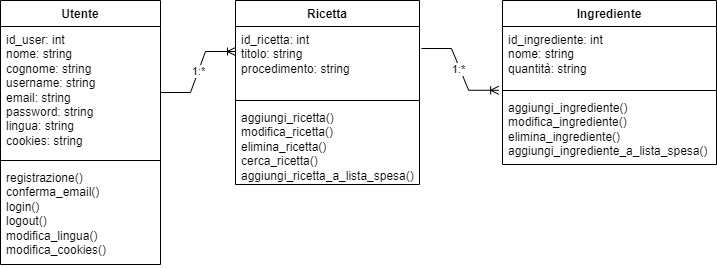
\includegraphics[width=11cm]{images/classricette.png}
  \captionof{figure}{Classi Ricetta e Ingrediente}
\end{center}
\section{Ricetta}

La classe {\sffamily Ricetta} permette di descrivere gli oggetti che rappresentano le ricette dell'utente e descrive le operazione possibili per ogni oggetto di questo tipo. 
\subsubsection*{Attributi}
\begin{itemize} \setlength\itemsep{0.01em}
\item {\ttfamily id\_ricetta}: intero contenente un numero progressivo che identifica la precisa ricetta.
\item {\ttfamily titolo}: stringa contenente il titolo che l'utente sceglie di dare alla ricetta.
\item {\ttfamily procedimento}: stringa contenente un testo che comprende il procedimento ed eventuali note.
\end{itemize}
\subsubsection*{Metodi}
\begin{itemize} \setlength\itemsep{0.01em}
\item {\ttfamily aggiungi\_ricetta}: metodo che l'utente invoca quando deve creare una nuova ricetta. Il sistema, attraverso tal funzione, la inserisce nel database.
\item {\ttfamily modifica\_ricetta}: metodo che l'utente invoca quando desidera modificare una ricetta.
\item {\ttfamily elimina\_ricetta}: metodo che l'utente invoca quando desidera cancellare una ricetta. L'eliminazione comporta anche l'eliminazione degli ingredienti ad essa associati.
\item {\ttfamily cerca\_ricetta}: metodo che l'utente invoca quando desidera cercare una ricetta. 
\item {\ttfamily aggiungi\_ricetta\_a\_lista\_spesa}: metodo che l'utente invoca quando desidera aggiungere tutti gli ingredienti alla propria lista della spesa. 

\end{itemize}
\subsubsection*{Object Constraint Language (OCL)}
\begin{itemize}
\item {\ttfamily context Ricetta inv TitoloLunghezza: self.titolo.size() >= 1}
\item {\ttfamily context Ricetta::aggiungi\_ricetta() \\pre self.titolo->notEmpty()}

\end{itemize}
\section{Ingrediente}

La classe {\sffamily Ingrediente} permette di descrivere gli oggetti che rappresentano gli ingredienti di una ricetta e descrive le operazione possibili per ogni oggetto di questo tipo.
\subsubsection*{Attributi}
\begin{itemize} \setlength\itemsep{0.01em}
\item {\ttfamily id\_ingrediente}: intero contenente l'identificativo dell'ingrediente.
\item {\ttfamily nome}: stringa contenente l'ingrediente.
\item {\ttfamily quantità}: stringa contenente la quantità dell'ingrediente nel contesto della ricetta
\end{itemize}
\subsubsection*{Metodi}
\begin{itemize} \setlength\itemsep{0.01em}
\item {\ttfamily aggiungi\_ingrediente}: metodo che l'utente invoca quando deve inserire un nuovo ingrediente. 
\item {\ttfamily modifica\_ingrediente}: metodo che l'utente invoca quando desidera modificare le informazioni relative ad un ingrediente.
\item {\ttfamily elimina\_ingrediente}: metodo che l'utente invoca quando desidera eliminare un ingrediente. 
\item {\ttfamily aggiungi\_ingrediente\_a\_lista\_spesa}: metodo che l'utente invoca quando desidera aggiungere l'ingrediente alla propria lista della spesa. 
\end{itemize}
\subsubsection*{Object Constraint Language (OCL)}
\begin{itemize}
\item {\ttfamily context Ingrediente inv NomeLunghezza: self.nome.size() >= 1}
\item {\ttfamily context Ingrediente::aggiungi\_ingrediente() \\pre self.nome->notEmpty()}

\end{itemize}
\newpage


\begin{center}
  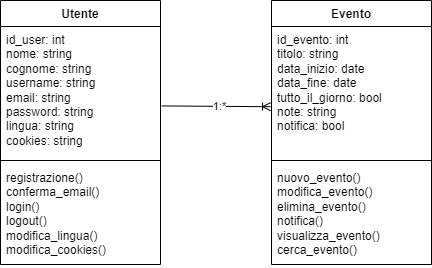
\includegraphics[width=7cm]{images/classeventi.png}
  \captionof{figure}{Classe Evento}
\end{center}
\section{Evento}
La classe {\sffamily Evento} permette di descrivere gli oggetti che rappresentano gli eventi e descrive le operazione possibili per ogni oggetto di questo tipo.
\subsubsection*{Attributi}
\begin{itemize} \setlength\itemsep{0.01em}
\item {\ttfamily id\_evento}: intero identificativo dell'evento specifico.
\item {\ttfamily titolo}: stringa contenente il titolo che l'utente desidera associare ad un evento.
\item {\ttfamily data\_inizio}: data (secondo il formato dato dalla classe {\sffamily Data}) in cui l'evento inizia.
\item {\ttfamily data\_fine}: data (secondo il formato dato dalla classe {\sffamily Data}) in cui l'evento termina.
\item {\ttfamily tutto\_il\_giorno}: booleano che identifica se l'evento è relativo ad una giornata intera (da mezzanotte a mezzanotte).
\item {\ttfamily note}: stringa contenente le note che l'utente desidera inserire.
\item {\ttfamily notifica}: booleano in cui è memorizzata la scelta dell'utente in merito al ricevere la notifica.
\end{itemize}
\subsubsection*{Metodi}
\begin{itemize} \setlength\itemsep{0.01em}
\item {\ttfamily nuovo\_evento}: metodo che l'utente invoca quando deve inserire un nuovo evento.
\item {\ttfamily modifica\_evento}: metodo che l'utente invoca quando desidera modificare qualunque attributo dell'evento.
\item {\ttfamily elimina\_evento}: metodo che l'utente invoca quando desidera eliminare un evento. 
\item {\ttfamily visualizza\_evento}: metodo che l'utente invoca quando desidera visualizzare l'evento.
\item {\ttfamily cerca\_evento}: metodo che l'utente invoca quando desidera cercare un evento.
\item {\ttfamily notifica}: metodo invocato quando l'utente riceve la notifica di un evento.
\end{itemize}
\subsubsection*{Object Constraint Language (OCL)}
\begin{itemize}
\item {\ttfamily context Evento inv self.data\_fine > self.data\_fine}
\item {\ttfamily context Evento inv NomeLunghezza: self.titolo.size() >= 1}
\item {\ttfamily context Evento::aggiungi\_evento() \\pre self.titolo->notEmpty()}

\end{itemize}
\newpage
\begin{center}
  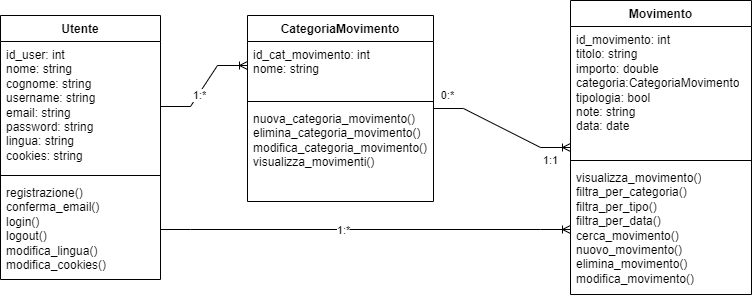
\includegraphics[width=11cm]{images/classbudget.png}
  \captionof{figure}{Classi Movimento e CategoriaMovimento}
\end{center}
\section{Categoria Movimento}

La classe {\sffamily CategoriaMovimento} permette di descrivere gli oggetti che rappresentano le categorie con cui l'utente classifica i propri movimenti e descrive le operazione possibili per ogni oggetto di questo tipo.
\subsubsection*{Attributi}
\begin{itemize} \setlength\itemsep{0.01em}
\item {\ttfamily id\_cat\_movimento}: intero contenente un numero progressivo che identifica la precisa categoria.
\item {\ttfamily nome}: stringa contenente il nome che l'utente sceglie di dare alla categoria.
\end{itemize}
\subsubsection*{Metodi}
\begin{itemize} \setlength\itemsep{0.01em}
\item {\ttfamily nuova\_categoria\_movimento}: metodo che l'utente invoca quando deve creare una nuova categoria. Il sistema, attraverso tal funzione, la inserisce nel database.
\item {\ttfamily modifica\_categoria\_movimento}: metodo che l'utente invoca quando desidera modificare il nome di una categoria.
\item {\ttfamily elimina\_categoria\_movimento}: metodo che l'utente invoca quando desidera cancellare una categoria. L'eliminazione non comporta la cancellazione dei movimenti associati alla categoria.
\item {\ttfamily visualizza\_movimenti}: metodo consente all'utente di visualizzare tutti i movimenti associati alla categoria.
\end{itemize}
\subsubsection*{Object Constraint Language (OCL)}
\begin{itemize}
\item {\ttfamily context CategoriaMovimento inv NomeLunghezza: self.nome.size() >= 1}
\item {\ttfamily context CategoriaMovimento::nuova\_categoria\_movimento() \\pre self.nome->notEmpty()}

\end{itemize}
\section{Movimento}

La classe {\sffamily Movimento} permette di descrivere gli oggetti che rappresentano i movimenti e descrive le operazioni possibili per ogni oggetto di questo tipo.
\subsubsection*{Attributi}
\begin{itemize} \setlength\itemsep{0.01em}
\item {\ttfamily id\_movimento}: intero contenente un numero progressivo che identifica il preciso movimento.
\item {\ttfamily titolo}: stringa contenente il titolo del movimento.
\item {\ttfamily importo}: valore numerico associato all'importo.
\item {\ttfamily categoria}:  categoria a cui il movimento è associato.
\item {\ttfamily tipologia}: booleano contenente la tipologia del moovimento (entrata o uscita).
\item {\ttfamily note}: stringa contenente le note che l'utente desidera inserire.
\item {\ttfamily data}: data (secondo il formato dato dalla classe {\sffamily Data}) associata al movimento.
\end{itemize}
\subsubsection*{Metodi}
\begin{itemize} \setlength\itemsep{0.01em}
\item {\ttfamily nuovo\_movimento}: metodo che l'utente invoca quando deve inserire un nuovo movimento. 
\item {\ttfamily modifica\_movimento}: metodo che l'utente invoca quando desidera modificare qualunque attributo del movimento.
\item {\ttfamily elimina\_movimento}: metodo che l'utente invoca quando desidera eliminare un movimento. 
\item {\ttfamily visualizza\_movimento}: metodo che l'utente invoca quando desidera mostrare i dati relativi al movimento
\item {\ttfamily cerca\_moovimento}: metodo che l'utente invoca quando desidera cercare un movimento. 
\item {\ttfamily filtra\_per\_categoria}: metodo che l'utente invoca quando desidera mostrare tutti i movimenti di una specifica categoria. 
\item {\ttfamily filtra\_per\_tipo}: metodo che l'utente invoca quando desidera mostrare tutti i movimenti di un tipo specifico (tutte le entrate o tutte le uscite). 
\item {\ttfamily filtra\_per\_data}: metodo che l'utente invoca quando desidera mostrare tutti i movimenti dell'ultimo mese. 
\end{itemize}
\subsubsection*{Object Constraint Language (OCL)}
\begin{itemize}
\item {\ttfamily context Movimento inv TitoloLunghezza: self.titolo.size() >= 1}
\item {\ttfamily context Movimento::nuovo\_movimento() \\pre self.titolo->notEmpty() \\pre self.importo->notEmpty()}

\end{itemize}

\newpage

\begin{center}
  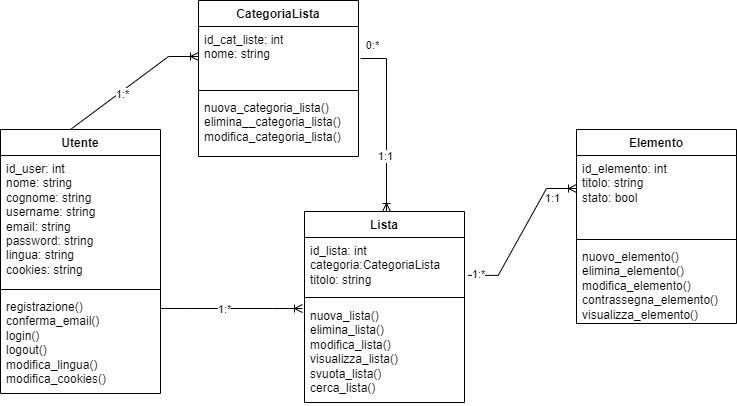
\includegraphics[width=16cm]{images/classliste.png}
  \captionof{figure}{Classi CategoriaLista, Lista ed Elemento}
\end{center}
\section{Categoria Lista}

La classe {\sffamily CategoriaLista} permette di descrivere gli oggetti che rappresentano le categorie con cui l'utente classifica le proprie liste e descrive le operazione possibili per ogni oggetto di questo tipo.
\subsubsection*{Attributi}
\begin{itemize} \setlength\itemsep{0.01em}
\item {\ttfamily id\_cat\_lista}: intero contenente un numero progressivo che identifica la precisa categoria.
\item {\ttfamily nome}: stringa contenente il nome che l'utente sceglie di dare alla categoria.
\end{itemize}
\subsubsection*{Metodi}
\begin{itemize} \setlength\itemsep{0.01em}
\item {\ttfamily nuova\_categoria\_lista}: metodo che l'utente invoca quando deve creare una nuova categoria.
\item {\ttfamily modifica\_categoria\_lista}: metodo che l'utente invoca quando desidera modificare il nome di una categoria.
\item {\ttfamily elimina\_categoria\_lista}: metodo che l'utente invoca quando desidera cancellare una categoria. L'eliminazione non comporta la cancellazione delle liste associate alla categoria.
\end{itemize}
\subsubsection*{Object Constraint Language (OCL)}
\begin{itemize}
\item {\ttfamily context CategoriaLista inv NomeLunghezza: self.nome.size() >= 1}
\item {\ttfamily context CategoriaLIsta::nuova\_categoria\_lista() \\pre self.nome->notEmpty()}

\end{itemize}
\section{Lista}

La classe {\sffamily Lista} permette di descrivere gli oggetti che rappresentano le liste con cui l'utente classifica i propri luoghi e descrive le operazione possibili per ogni oggetto di questo tipo.
\subsubsection*{Attributi}
\begin{itemize} \setlength\itemsep{0.01em}
\item {\ttfamily categoria}: categoria a cui è associata la lista.
\item {\ttfamily id\_lista}: intero contenente un numero progressivo che identifica la lista.
\item {\ttfamily titolo}: stringa contenente il titolo della lista.
\end{itemize}
\subsubsection*{Metodi}
\begin{itemize} \setlength\itemsep{0.01em}
\item {\ttfamily nuova\_lista}: metodo che l'utente invoca quando deve inserire una nuova lista. 
\item {\ttfamily modifica\_lista}: metodo che l'utente invoca quando desidera modificare una lista.
\item {\ttfamily elimina\_lista}: metodo che l'utente invoca quando desidera eliminare una lista. L'eliminazione comporta anche la cancellazione degli elementi associati.
\item {\ttfamily visualizza\_lista}: metodo che l'utente invoca quando desidera mostrare la lista e tutti gli elementi.
\item {\ttfamily cerca\_lista}: metodo che l'utente invoca quando desidera cercare una lista. 
\item {\ttfamily svuota\_lista}: metodo che l'utente invoca quando desidera eliminare tutti gli elementi della lista senza però cancellare la lista. 
\end{itemize}
\subsubsection*{Object Constraint Language (OCL)}
\begin{itemize}
\item {\ttfamily context Lista inv TitoloLunghezza: self.titolo.size() >= 1}
\item {\ttfamily context Lista::nuova\_lista() \\pre self.titolo->notEmpty() }

\end{itemize}
\section{Elemento}

La classe {\sffamily Elemento} permette di descrivere gli oggetti che rappresentano gli elementi della lista e descrive le operazione possibili per ogni oggetto di questo tipo.
\subsubsection*{Attributi}
\begin{itemize} \setlength\itemsep{0.01em}
\item {\ttfamily id\_elemento}: intero contenente un numero progressivo che identifica l'elemento.
\item {\ttfamily titolo}: stringa contenente il titolo dell'elemento.
\item {\ttfamily stato}: booleano che identifica lo stato dell'elemento (contrassegnato o non contrassegnato).
\end{itemize}
\subsubsection*{Metodi}
\begin{itemize} \setlength\itemsep{0.01em}
\item {\ttfamily nuovo\_elemento}: metodo che l'utente invoca quando deve inserire un nuovo elemento. 
\item {\ttfamily modifica\_elemento}: metodo che l'utente invoca quando desidera modificare un elemento.
\item {\ttfamily elimina\_elemento}: metodo che l'utente invoca quando desidera eliminare un elemento. 
\item {\ttfamily visualizza\_elemento}: metodo che l'utente invoca quando desidera mostrare l'elemento.
\item {\ttfamily contrassegna\_elemento}: metodo che l'utente invoca quando desidera contrassegnare un elemento. 
\end{itemize}
\subsubsection*{Object Constraint Language (OCL)}
\begin{itemize}
\item {\ttfamily context Elemento inv TitoloLunghezza: self.titolo.size() >= 1}
\item {\ttfamily context Elemento::nuovo\_elemento() \\pre self.titolo->notEmpty() }
\item {\ttfamily context Elemento::contrassegna\_elemento() \\post self.stato = true }

\end{itemize}



%_{_{_{_{_{_{_{_{_{_{_{_{_{_{_{_{_{_{_{_{ALLA FINE_{_{_{_{}}}}}_{_{_{_{_{}}}}}}
\vspace{15cm}
\hrule
\vspace{0.5cm}


Mauro Meneghello - matricola 217564 - mauro.meneghello@studenti.unitn.it

Luca Boschiero - matricola 217460 -  luca.boschiero@studenti.unitn.it

Nicola Turniano - matricola 217457 - nicola.turniano@studenti.unitn.it

%-----------------------------------------
 \end{document}